\documentclass[11pt,a4paper]{article}
\usepackage[utf8]{inputenc}
\usepackage{amsmath,amssymb}
\usepackage{xcolor}
\usepackage{hyperref}
\usepackage{booktabs}
\usepackage{enumitem}
\usepackage[margin=1in]{geometry}
\usepackage{longtable}
\usepackage{titlesec}
\usepackage{fancyhdr}
\usepackage{tikz}
\usetikzlibrary{arrows.meta,positioning,decorations.pathreplacing}
\usepackage{mathtools}

\hypersetup{
  colorlinks=true,
  linkcolor=blue!70!black,
  urlcolor=blue!60!black,
  citecolor=blue!70!black
}

\pagestyle{fancy}
\fancyhead[L]{\small Constructive Reverse Mathematics Series}
\fancyhead[R]{\small Paul Chun-Kit Lee}
\fancyfoot[C]{\thepage}

\titleformat{\section}{\large\bfseries}{Paper \thesection:}{0.5em}{}
\titleformat{\subsection}{\normalsize\itshape}{}{0em}{}

\setcounter{section}{0}

\title{\LARGE\bfseries Constructive Reverse Mathematics Series\\[0.3em]
\Large Series Guide: Papers 1--71 with Abstracts}
\author{Paul Chun-Kit Lee\\New York University\\
\texttt{dr.paul.c.lee@gmail.com}}
\date{February 2026\\[0.5em]
\normalsize Series DOI: \href{https://doi.org/10.5281/zenodo.17054050}{10.5281/zenodo.17054050}}

\begin{document}
\maketitle
\thispagestyle{empty}

\begin{abstract}
\noindent This booklet collects the titles and abstracts of all 69 active papers (of 71 numbered) in the Constructive Reverse Mathematics (CRM) series. The programme calibrates the logical strength of theorems across mathematical physics and arithmetic geometry against the constructive hierarchy: BISH $\subset$ BISH+LLPO $\subset$ BISH+WLPO $\subset$ BISH+LPO $\subset$ CLASS, with independent axes for Markov's Principle (MP), the Fan Theorem (FT), and Dependent Choice (DC). The main finding is that all empirically accessible predictions in known physics require exactly BISH+LPO. Papers 45--68 extend this to arithmetic geometry and number theory, establishing the Decidable Polarized Tannakian (DPT) framework, the three-invariant hierarchy (rank, Hodge level, Lang constant), and the CRM audit of Wiles's proof of Fermat's Last Theorem. Approximately 87,000 lines of Lean~4 code formalize the results.
\end{abstract}

\tableofcontents
\newpage

%=============================================================================
% PROGRAMME OVERVIEW
%=============================================================================
\part*{Programme Overview}
\addcontentsline{toc}{part}{Programme Overview}

\subsection*{What is Constructive Reverse Mathematics?}

Constructive Reverse Mathematics (CRM) calibrates the logical strength of mathematical theorems against a hierarchy of constructive principles.  Rather than asking ``is this theorem true?'', CRM asks ``what non-constructive resources does this theorem \emph{require}?''  The answer is a position in the hierarchy
\[
\mathrm{BISH} \;\subset\; \mathrm{BISH{+}LLPO} \;\subset\; \mathrm{BISH{+}WLPO} \;\subset\; \mathrm{BISH{+}LPO} \;\subset\; \mathrm{CLASS},
\]
with independent axes for Markov's Principle (MP), the Fan Theorem (FT), and Dependent Choice (DC).

\begin{itemize}[nosep]
\item \textbf{BISH} (Bishop's constructive mathematics): the base system, requiring explicit witnesses for all existence claims.
\item \textbf{LLPO} (Lesser Limited Principle of Omniscience): decides disjunctions over binary sequences.
\item \textbf{WLPO} (Weak Limited Principle of Omniscience): decides whether a binary sequence is identically zero.
\item \textbf{LPO} (Limited Principle of Omniscience): decides whether a binary sequence contains a 1.
\item \textbf{MP} (Markov's Principle): if a computation cannot fail to halt, then it halts. Orthogonal to the omniscience spine.
\item \textbf{FT} (Fan Theorem): every bar on Cantor space is uniform.  Independent of the omniscience spine.
\item \textbf{DC} (Dependent Choice): sequential choice along a total relation.  Independent of omniscience and FT.
\end{itemize}

\subsection*{The programme in three phases}

\textbf{Phase I: Mathematical Physics (Papers 1--44).}  Systematic calibration of theorems across functional analysis, quantum mechanics, general relativity, statistical mechanics, QFT, quantum information, classical mechanics, cosmology, and quantum foundations.  The main finding: \emph{all empirically accessible predictions in known physics require exactly $\mathrm{BISH{+}LPO}$}.  The Fan Theorem and Dependent Choice are physically dispensable (Papers~30--31).  The LPO cost is genuine and instantiated by Fekete's Subadditive Lemma (Paper~29).

\textbf{Phase II: Arithmetic Geometry (Papers 45--66).}  Extension to the Hodge, Tate, BSD, Fontaine--Mazur, and Weight-Monodromy conjectures.  Each conjecture exhibits a \emph{de-omniscientizing descent}: geometric origin converts LPO-dependent claims to BISH-decidable ones.  The Decidable Polarized Tannakian (DPT) framework (Paper~50) axiomatizes this pattern.  Three invariants---analytic rank, Hodge level, Lang constant---classify the logical cost of cycle-search for any motive.

\textbf{Phase III: Synthesis (Papers 67--71).}  The arithmetic geometry monograph (Paper~67), the CRM audit of Fermat's Last Theorem (Paper~68, result: BISH), the function field Langlands audit (Paper~69, result: BISH), the capstone Archimedean Principle (Paper~70), and engineering applications to lattice cryptography (Paper~71).  The capstone finding: \emph{the real numbers are the sole source of logical difficulty in both mathematical physics and arithmetic geometry}, via the mechanism $u(\mathbb{R})=\infty$.

%=============================================================================
% LOGICAL HIERARCHY DIAGRAM
%=============================================================================
\newpage
\subsection*{The Logical Hierarchy}
\addcontentsline{toc}{section}{The Logical Hierarchy}

\begin{figure}[ht]
\centering
\resizebox{\textwidth}{!}{%
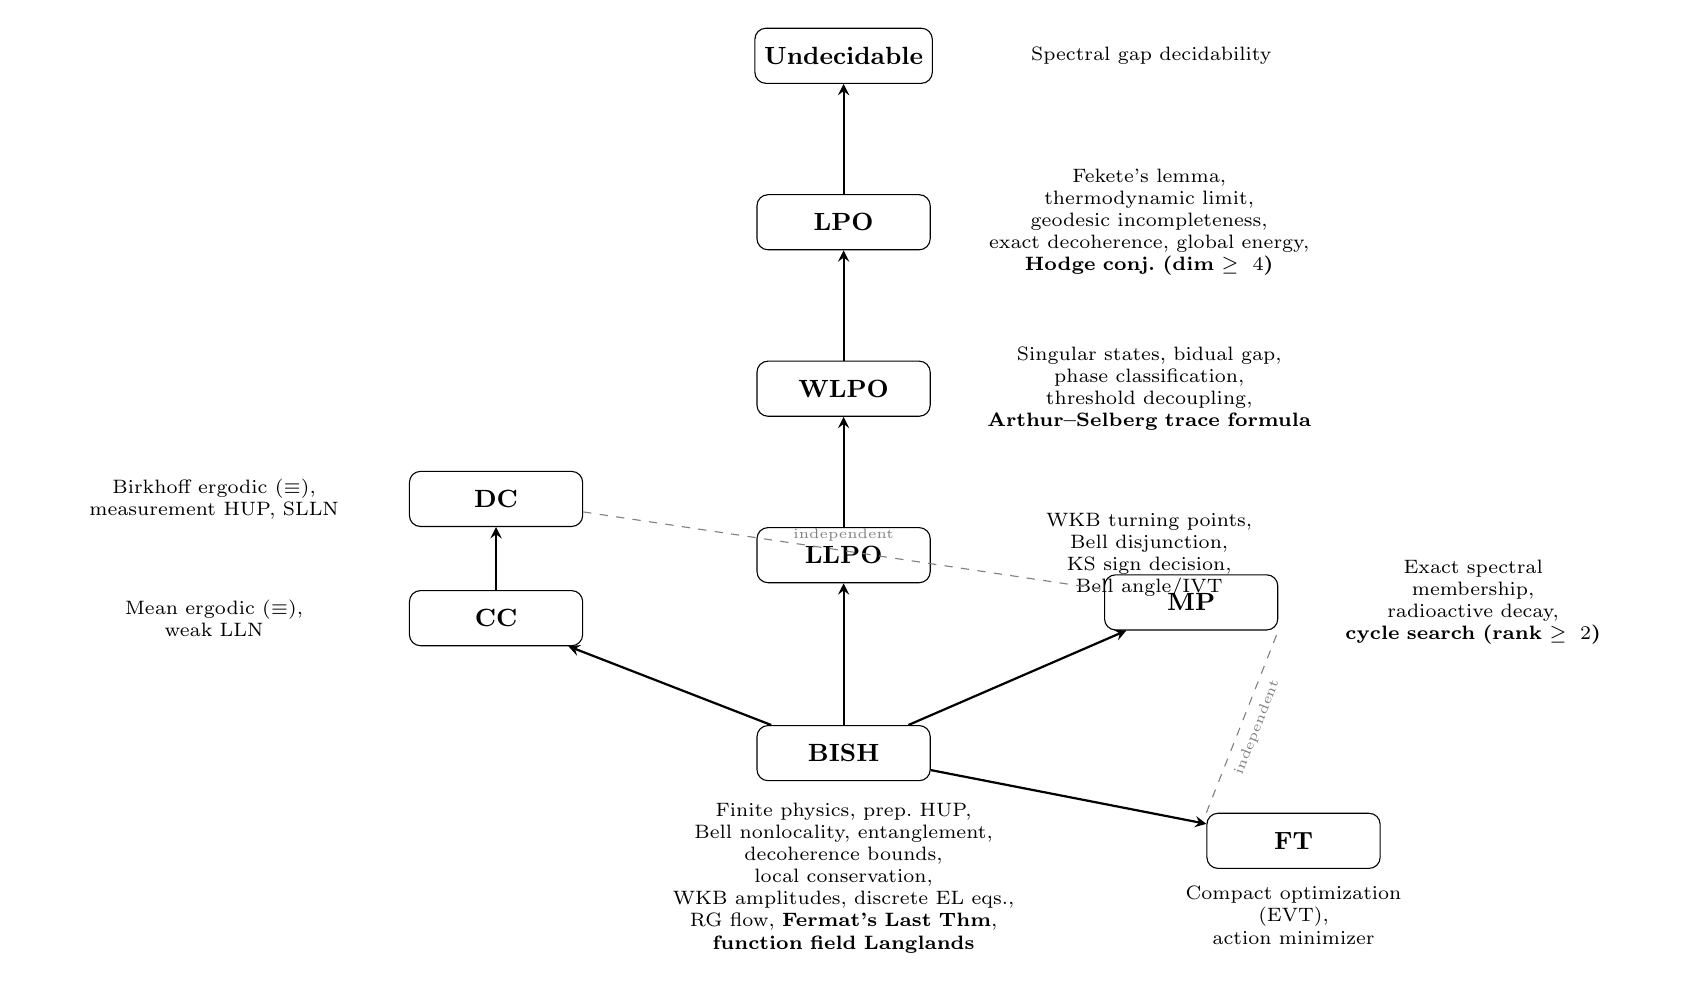
\begin{tikzpicture}[
  node distance=1.4cm and 2.8cm,
  principle/.style={draw, rounded corners, minimum width=2.2cm, minimum height=0.7cm, font=\small\bfseries},
  physlabel/.style={font=\scriptsize, text width=4.5cm, align=center},
  >=stealth
]
% Main spine
\node[principle] (bish) {BISH};
\node[principle, above=1.8cm of bish] (llpo) {LLPO};
\node[principle, above=of llpo] (wlpo) {WLPO};
\node[principle, above=of wlpo] (lpo) {LPO};
\node[principle, above=of lpo] (undec) {Undecidable};

% Choice hierarchy
\node[principle, above left=1.0cm and 2.2cm of bish] (cc) {CC};
\node[principle, above=0.8cm of cc] (dc) {DC};
% Orthogonal branch
\node[principle, above right=1.2cm and 2.2cm of bish] (mp) {MP};

% Fan Theorem: independent branch
\node[principle, below right=0.4cm and 3.5cm of bish] (ft) {FT};

% Edges (Hasse diagram)
\draw[thick, ->] (bish) -- (cc);
\draw[thick, ->] (cc) -- (dc);
\draw[thick, ->] (bish) -- (mp);
\draw[thick, ->] (bish) -- (llpo);
\draw[thick, ->] (llpo) -- (wlpo);
\draw[thick, ->] (wlpo) -- (lpo);
\draw[thick, ->] (lpo) -- (undec);
\draw[thick, ->] (bish) -- (ft);

% Physical labels
\node[physlabel, below=0.15cm of bish] {Finite physics, prep.\ HUP,\\Bell nonlocality, entanglement,\\decoherence bounds, local conservation,\\WKB amplitudes, discrete EL eqs.,\\RG flow, \textbf{Fermat's Last Thm},\\\textbf{function field Langlands}};
\node[physlabel, left=0.1cm of cc] {Mean ergodic ($\equiv$),\\weak LLN};
\node[physlabel, left=0.1cm of dc] {Birkhoff ergodic ($\equiv$),\\measurement HUP, SLLN};
\node[physlabel, right=0.1cm of mp] {Exact spectral\\membership,\\radioactive decay,\\\textbf{cycle search (rank $\geq2$)}};
\node[physlabel, right=0.4cm of llpo] {WKB turning points,\\Bell disjunction,\\KS sign decision,\\Bell angle/IVT};
\node[physlabel, right=0.4cm of wlpo] {Singular states, bidual gap,\\phase classification,\\threshold decoupling,\\\textbf{Arthur--Selberg trace formula}};
\node[physlabel, right=0.4cm of lpo] {Fekete's lemma,\\thermodynamic limit,\\geodesic incompleteness,\\exact decoherence, global energy,\\\textbf{Hodge conj.\ (dim $\geq4$)}};
\node[physlabel, right=0.4cm of undec] {Spectral gap decidability};
\node[physlabel, below=0.1cm of ft] {Compact optimization\\(EVT),\\action minimizer};

% Independence annotations
\draw[dashed, gray] (dc) -- node[above, font=\tiny, gray] {independent} (mp);
\draw[dashed, gray] (ft.north west) -- node[below, font=\tiny, gray, sloped] {independent} (mp.south east);

\end{tikzpicture}%
}
\caption{The logical geography of the CRM programme (Papers~1--71).  Arrows indicate strict implication over BISH.  The omniscience spine (BISH $<$ LLPO $<$ WLPO $<$ LPO) is the dominant vertical chain.  DC and MP occupy orthogonal positions.  FT is a third independent branch.  \textbf{Bold entries} are from the arithmetic geometry and synthesis phases.}
\label{fig:hierarchy}
\end{figure}

%=============================================================================
% MASTER CALIBRATION TABLE
%=============================================================================
\newpage
\subsection*{Master Calibration Table}
\addcontentsline{toc}{section}{Master Calibration Table}

The table below collects calibrated entries from 71 papers spanning mathematical physics, arithmetic geometry, and the Langlands programme.

\begin{center}
\begin{longtable}{@{}p{5.8cm}ll@{}}
\toprule
\textbf{Theorem / Result} & \textbf{Level} & \textbf{Source} \\
\midrule
\endfirsthead
\toprule
\textbf{Theorem / Result} & \textbf{Level} & \textbf{Source} \\
\midrule
\endhead
\multicolumn{3}{l}{\textit{BISH (fully constructive):}} \\
Finite-volume physics, finite-size bounds & BISH & Papers 8, 9 \\
Preparation uncertainty (HUP) & BISH & Paper 6 \\
Bell nonlocality (CHSH/Tsirelson) & BISH & Paper 11 \\
Entanglement entropy & BISH & Paper 11 \\
Schwarzschild interior (finite-time) & BISH & Paper 13 \\
Decoherence bounds (finite-step) & BISH & Paper 14 \\
Local conservation (Noether) & BISH & Paper 15 \\
Born probability (finite-dim) & BISH & Paper 16 \\
BH entropy (algebraic correction) & BISH & Paper 17 \\
WKB amplitude (specific barriers) & BISH & Paper 19 \\
Discrete Euler--Lagrange equations & BISH & Paper 28 \\
Yukawa RG one-loop flow & BISH & Paper 18 \\
QED Landau pole, Ward--Takahashi & BISH & Paper 32 \\
Fixed-order scattering (Bhabha) & BISH & Paper 34 \\
Hodge polarization degeneration & BISH & Paper 45 \\
Algebraic cycle verification & BISH & Paper 49 \\
CM elliptic motives (decidable) & BISH & Paper 53 \\
Fermat's Last Theorem & BISH & Paper 68 \\
Function field Langlands ($\mathrm{GL}_n$, gen.\ $G$) & BISH & Paper 69 \\
Lattice cryptography (LLL, exp.\ approx.) & BISH & Paper 71 \\
\midrule
\multicolumn{3}{l}{\textit{Choice hierarchy (CC $<$ DC):}} \\
Mean ergodic theorem & $\equiv$ CC & Paper 25 \\
Birkhoff's ergodic theorem & $\equiv$ DC & Paper 25 \\
Frequentist convergence (SLLN) & $\leq$ DC & Papers 16, 25 \\
\midrule
\multicolumn{3}{l}{\textit{LLPO:}} \\
WKB turning-point decision (IVT) & $\equiv$ LLPO & Paper 19 \\
Bell disjunctive conclusion & $\equiv$ LLPO & Paper 21 \\
KS sign decision (contextuality) & $\equiv$ LLPO & Paper 24 \\
Bell angle optimisation (IVT) & $\equiv$ LLPO & Paper 27 \\
\midrule
\multicolumn{3}{l}{\textit{MP (Markov's Principle):}} \\
Exact spectral membership & MP & Paper 4 \\
Radioactive decay (eventual detection) & $\equiv$ MP & Paper 22 \\
Cycle search, rank $\geq 2$ (without Lang) & MP & Paper 61 \\
SVP polynomial approx.\ (BKZ) & BISH+MP & Paper 71 \\
\midrule
\multicolumn{3}{l}{\textit{WLPO:}} \\
Bidual-gap / singular states & $\equiv$ WLPO & Papers 2, 7 \\
Phase classification (magnetization) & $\equiv$ WLPO & Paper 20 \\
Step-function threshold decoupling & WLPO & Paper 18 \\
Arthur--Selberg trace formula & WLPO & Paper 68 \\
\midrule
\multicolumn{3}{l}{\textit{FT (Fan Theorem) --- physically dispensable:}} \\
Compact optimization (EVT on $[a,b]$) & $\equiv$ FT & Paper 23 \\
Action minimizer existence (variational) & $\equiv$ FT & Paper 28 \\
\midrule
\multicolumn{3}{l}{\textit{LPO:}} \\
Thermodynamic limit existence & $\equiv$ LPO & Papers 8, 9, 29 \\
Fekete's lemma (subadditive sequences) & $\equiv$ LPO & Paper 29 \\
Geodesic incompleteness (completed limit) & $\equiv$ LPO & Paper 13 \\
Exact decoherence (wave fn collapse) & $\equiv$ LPO & Paper 14 \\
Global energy (infinite-volume) & $\equiv$ LPO & Paper 15 \\
BH entropy density convergence & $\equiv$ LPO & Paper 17 \\
Galois-invariance decidability ($\mathbb{Q}_\ell$) & $\equiv$ LPO & Paper 46 \\
$L(E,1)=0$ decision & $\equiv$ LPO & Paper 48 \\
Hodge type $(r,r)$ decidability ($\mathbb{C}$) & $\equiv$ LPO & Paper 49 \\
\midrule
\multicolumn{3}{l}{\textit{Undecidable:}} \\
Spectral gap decidability & $\Sigma_1^0$-complete & Cubitt et al. \\
Generic spectral gap (no promise) & $\Sigma_2^0$-complete & Paper 39 \\
\bottomrule
\end{longtable}
\end{center}

%=============================================================================
% DPT FRAMEWORK
%=============================================================================
\subsection*{The DPT Framework (Paper 50)}
\addcontentsline{toc}{section}{The DPT Framework}

A \emph{Decidable Polarized Tannakian} (DPT) category over $\mathbb{Q}$ is a $\mathbb{Q}$-linear abelian symmetric monoidal category $\mathcal{C}$ equipped with three axioms:

\begin{description}[style=unboxed,leftmargin=1em]
\item[Axiom 1 (Decidable morphisms --- Standard Conjecture D).] For all $X, Y \in \mathcal{C}$, the morphism space $\mathrm{Hom}(X,Y)$ has decidable equality: $\forall f,g\colon X \to Y,\; f = g \lor f \neq g$.

\item[Axiom 2 (Algebraic spectrum).] Every endomorphism $f \in \mathrm{End}(X)$ satisfies a monic polynomial $p \in \mathbb{Z}[t]$, forcing eigenvalues into $\overline{\mathbb{Q}}$.

\item[Axiom 3 (Archimedean polarization).] A faithful functor to real vector spaces equipped with a positive-definite bilinear form: $\langle x, x \rangle > 0$ for all $x \neq 0$.
\end{description}

\noindent Five conjectures (Hodge, Tate, BSD, Fontaine--Mazur, Weight-Monodromy) exhibit a uniform \emph{de-omniscientizing descent}: geometric origin converts LPO-dependent data to BISH-decidable numerical equivalence, mediated by the DPT axioms.

%=============================================================================
% ARCHIMEDEAN PRINCIPLE
%=============================================================================
\subsection*{The Archimedean Principle (Paper 70)}
\addcontentsline{toc}{section}{The Archimedean Principle}

\begin{figure}[ht]
\centering
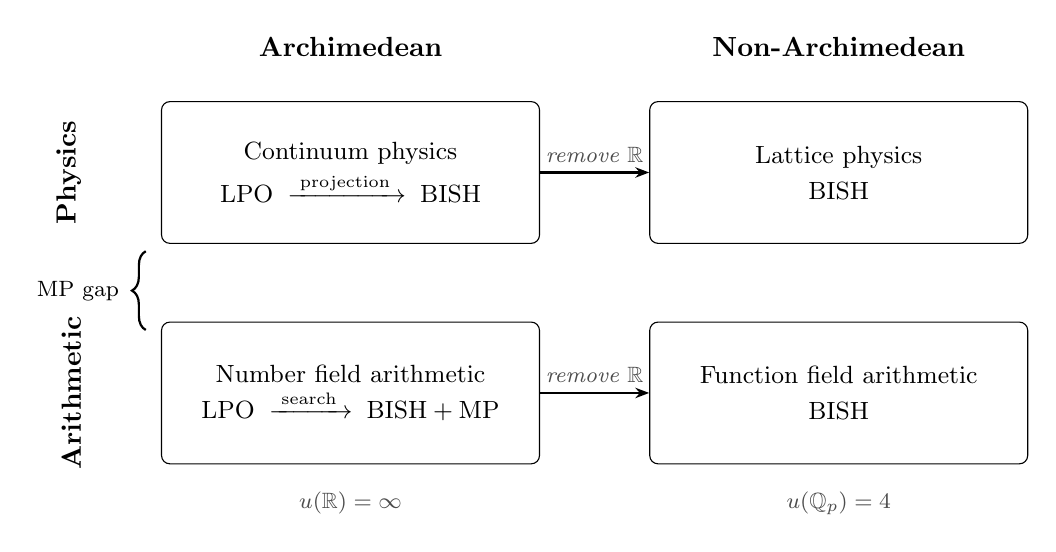
\begin{tikzpicture}[
    box/.style={draw, rounded corners=3pt, minimum width=4.8cm,
                minimum height=1.8cm, align=center, font=\small},
    arr/.style={-{Stealth[length=5pt]}, thick},
    ann/.style={font=\footnotesize\itshape, text=black!70}
  ]
  % Column headers
  \node[font=\bfseries] at (0, 2.6) {Archimedean};
  \node[font=\bfseries] at (6.2, 2.6) {Non-Archimedean};
  % Row headers
  \node[font=\bfseries, rotate=90, anchor=south] at (-3.3, 1.0) {Physics};
  \node[font=\bfseries, rotate=90, anchor=south] at (-3.3,-1.8) {Arithmetic};
  % Four boxes
  \node[box] (CP) at (0, 1.0)
    {Continuum physics\\[2pt] $\mathrm{LPO} \;\xrightarrow{\;\text{projection}\;}\; \mathrm{BISH}$};
  \node[box] (LP) at (6.2, 1.0)
    {Lattice physics\\[2pt] $\mathrm{BISH}$};
  \node[box] (NA) at (0,-1.8)
    {Number field arithmetic\\[2pt] $\mathrm{LPO} \;\xrightarrow{\;\text{search}\;}\; \mathrm{BISH} + \mathrm{MP}$};
  \node[box] (FA) at (6.2,-1.8)
    {Function field arithmetic\\[2pt] $\mathrm{BISH}$};
  % Horizontal arrows
  \draw[arr] (CP.east) -- (LP.west) node[midway,above,ann] {remove $\mathbb{R}$};
  \draw[arr] (NA.east) -- (FA.west) node[midway,above,ann] {remove $\mathbb{R}$};
  % u-invariant annotations
  \node[ann] at (0, -3.2) {$u(\mathbb{R}) = \infty$};
  \node[ann] at (6.2, -3.2) {$u(\mathbb{Q}_p) = 4$};
  % MP gap brace
  \draw[decorate, decoration={brace, amplitude=5pt, mirror}, thick]
    (-2.6, 0.0) -- (-2.6, -1.0)
    node[midway, left=6pt, font=\footnotesize] {MP gap};
\end{tikzpicture}
\caption{The four-domain parameterisation (Paper~70).  The CRM level is determined by one parameter: presence of the Archimedean place.  The descent type (projection vs.\ search) determines the residual.}
\label{fig:archimedean}
\end{figure}

\noindent The mechanism is $u(\mathbb{R}) = \infty$: the real numbers are the only completion of~$\mathbb{Q}$ where positive-definite forms exist in every dimension.  Three fields independently exploit this via the same architecture: \emph{Hilbert space inner product} (physics), \emph{Rosati involution} (arithmetic geometry), \emph{Petersson inner product} (automorphic forms).  Remove $\mathbb{R}$ and both physics and arithmetic collapse to BISH.  The difference between them is how they descend: physics uses \emph{projection} (eliminating MP), number theory uses \emph{search} (preserving MP as Diophantine hardness).

%=============================================================================
% FORMALIZATION STATISTICS
%=============================================================================
\subsection*{Formalization Statistics}
\addcontentsline{toc}{section}{Formalization Statistics}

\begin{center}
\begin{tabular}{@{}lr@{}}
\toprule
\textbf{Metric} & \textbf{Value} \\
\midrule
Total papers (numbered) & 71 \\
Active papers & 69 \\
Withdrawn & 2 (Papers 1, 3) \\
Retired (merged) & 2 (Papers 60, 62) \\
Papers with Zenodo DOI & 66 \\
Papers with Lean~4 formalization & $\sim$61 \\
Total Lean~4 lines & $\sim$88,000+ \\
Papers with zero \texttt{sorry} & $\geq$22 \\
Lean toolchain & v4.28.0-rc1 \\
Mathlib dependency & v4.28.0-rc1 \\
\midrule
\textbf{Domains covered} & \\
\midrule
\multicolumn{2}{l}{Functional Analysis, Quantum Mechanics, General Relativity,} \\
\multicolumn{2}{l}{Statistical Mechanics, QFT (QED/QCD), Quantum Information,} \\
\multicolumn{2}{l}{Classical Mechanics, Foundations, Undecidability, AdS/CFT,} \\
\multicolumn{2}{l}{Cosmology, Arithmetic Geometry, Motives, Number Theory,} \\
\multicolumn{2}{l}{Langlands Programme, Cryptography} \\
\bottomrule
\end{tabular}
\end{center}

\newpage

%=============================================================================
% PART I: FOUNDATIONS (Papers 1--6)
%=============================================================================
\part*{Part I: Foundations (Papers 1--6)}
\addcontentsline{toc}{part}{Part I: Foundations}

%-----------------------------------------------------------------------------
\setcounter{section}{0}
\section{Rank-One Toggle Kernel}
\label{sec:p1}
\textbf{Status:} Withdrawn.\\
\textbf{DOI:} ---

\bigskip
\noindent\textit{This paper has been withdrawn from the series.}

%-----------------------------------------------------------------------------
\section{The Bidual Gap and WLPO}
\label{sec:p2}
\textbf{DOI:} \href{https://doi.org/10.5281/zenodo.18501689}{10.5281/zenodo.18501689}

\bigskip
\noindent\textbf{Abstract.}
We formalize the bidual gap of Banach spaces and prove it is equivalent to WLPO (the Weak Limited Principle of Omniscience). Gap detection requires exactly WLPO; the witness space is $c_0$ (sequences vanishing at infinity). The formalization establishes that Banach space non-reflexivity detection is a constructively calibrated problem with precise logical cost.

%-----------------------------------------------------------------------------
\section{[Withdrawn]}
\label{sec:p3}
\textbf{Status:} Withdrawn.\\
\textbf{DOI:} ---

\bigskip
\noindent\textit{This paper has been withdrawn from the series.}

%-----------------------------------------------------------------------------
\section{Axiom Calibration for Quantum Spectra}
\label{sec:p4}
\textbf{DOI:} \href{https://doi.org/10.5281/zenodo.17118223}{10.5281/zenodo.17118223}

\bigskip
\noindent\textbf{Abstract.}
Five spectral properties---from approximate eigenvalues to exact membership---are stratified from BISH to WLPO+MP. This provides a complete calibration of quantum spectral theory against the constructive hierarchy, showing that different spectral questions about the same operator carry different logical costs.

%-----------------------------------------------------------------------------
\section{Schwarzschild Curvature Verification}
\label{sec:p5}
\textbf{DOI:} \href{https://doi.org/10.5281/zenodo.18489703}{10.5281/zenodo.18489703}

\bigskip
\noindent\textbf{Abstract.}
We make Axiom Calibration the organizing principle for a foundations-first study of General Relativity. The paper contributes three AxCal instruments for GR: (I)~witness families pinned to a fixed $\Sigma_0^{\mathrm{GR}}$ signature; (II)~proof-route flags and portal theorems; and (III)~HeightCertificates. We calibrate five loci: G1 (explicit vacuum checks, Height~0), G2 (Cauchy/MGHD), G3 (singularity theorems), G4 (maximal extensions), and G5 (computable evolution).

%-----------------------------------------------------------------------------
\section{Heisenberg Uncertainty Principle (v2, CRM over Mathlib)}
\label{sec:p6}
\textbf{DOI:} \href{https://doi.org/10.5281/zenodo.18519836}{10.5281/zenodo.18519836}

\bigskip
\noindent\textbf{Abstract.}
We formalize the Robertson--Schr\"odinger and Schr\"odinger uncertainty inequalities in Lean~4 using Mathlib's InnerProductSpace API, within the framework of Constructive Reverse Mathematics. Both preparation-uncertainty inequalities are proved at Height~0 (fully constructive) using Cauchy--Schwarz, centered-vector decomposition, and elementary complex-number identities---all drawn from Mathlib with zero custom axioms. Measurement uncertainty, which requires constructing infinite measurement histories, is calibrated at $\mathrm{DC}_\omega$-height.

%=============================================================================
% PART II: PHYSICAL CALIBRATIONS (Papers 7--28)
%=============================================================================
\newpage
\part*{Part II: Physical Calibrations (Papers 7--28)}
\addcontentsline{toc}{part}{Part II: Physical Calibrations}

%-----------------------------------------------------------------------------
\section{Physical Bidual Gap, Trace-Class Operators}
\label{sec:p7}
\textbf{DOI:} \href{https://doi.org/10.5281/zenodo.18527559}{10.5281/zenodo.18527559}

\bigskip
\noindent\textbf{Abstract.}
We present a Lean~4 formalization of the Physical Bidual Gap Theorem, establishing Banach space non-reflexivity of the trace-class operators $\mathcal{S}^1$ on a separable Hilbert space and showing that any constructive witness of this non-reflexivity implies WLPO. In the algebraic formulation of quantum mechanics, $\mathcal{S}^1$ is the natural state space; our result shows that the gap between physical density matrices and the ``generalized states'' in $(\mathcal{S}^1)^{**}$ is constructively inaccessible. The formalization comprises 754 lines of Lean~4 code across 8 files.

%-----------------------------------------------------------------------------
\section{1D Ising Model and LPO}
\label{sec:p8}
\textbf{DOI:} \href{https://doi.org/10.5281/zenodo.18516813}{10.5281/zenodo.18516813}

\bigskip
\noindent\textbf{Abstract.}
We prove two complementary results about the thermodynamic limit of the one-dimensional Ising model. (A)~The finite-size error bound $|f_N(\beta)-f_\infty(\beta)|\le(1/N)\tanh(\beta)^N$ is provable in BISH without any omniscience principle. (B)~The existence of the thermodynamic limit as a completed real number is equivalent over BISH to LPO, via bounded monotone convergence instantiated through the Ising free energy. Together: the LPO cost is genuine and dispensable. The combined formalization comprises 1374 lines of Lean across 18 modules with zero sorries.

%-----------------------------------------------------------------------------
\section{Ising Formulation-Invariance}
\label{sec:p9}
\textbf{DOI:} \href{https://doi.org/10.5281/zenodo.18517570}{10.5281/zenodo.18517570}

\bigskip
\noindent\textbf{Abstract.}
We prove that the logical cost of the thermodynamic limit for the 1D Ising model is formulation-invariant: the same axiom profile arises from a purely combinatorial derivation as from the transfer-matrix approach of Paper~8. Specifically, we re-derive (A)~BISH dispensability and (B)~LPO equivalence using only finite sums over $\{-1,+1\}^N$, the binomial parity sieve, and elementary hyperbolic function arithmetic. No transfer matrices, eigenvalues, or linear algebra are used. The formalization comprises 1319 lines across 18 modules with zero sorries.

%-----------------------------------------------------------------------------
\section{Logical Geography of Mathematical Physics}
\label{sec:p10}
\textbf{DOI:} \href{https://doi.org/10.5281/zenodo.18636180}{10.5281/zenodo.18636180}

\bigskip
\noindent\textbf{Abstract.}
This paper synthesizes the machine-verified results of the constructive calibration programme---spanning functional analysis, quantum spectra, general relativity, uncertainty relations, statistical mechanics, quantum information, decoherence, conservation laws, measurement statistics, quantum gravity, particle physics, semiclassical mechanics, quantum foundations, radioactive decay, ergodic theory, classical mechanics, and subadditive convergence---into a single interpretive framework. The calibration table contains approximately fifty entries spanning BISH to undecidable, populated by Lean~4 formalizations totalling approximately 25,400 lines of code across eleven domains.

%-----------------------------------------------------------------------------
\section{Entanglement, CHSH, Tsirelson Bound}
\label{sec:p11}
\textbf{DOI:} \href{https://doi.org/10.5281/zenodo.18527676}{10.5281/zenodo.18527676}

\bigskip
\noindent\textbf{Abstract.}
We provide a complete Lean~4 formalization of two foundational results in quantum information theory: (A)~the Tsirelson bound on the CHSH operator ($|\langle\psi,\mathrm{CHSH}\,\psi\rangle|\le 2\sqrt{2}$); and (B)~the entanglement entropy of the Bell singlet state ($S(\rho_A)=\log 2$). The formalization comprises 639 lines across 8 modules with zero sorry.

%-----------------------------------------------------------------------------
\section{Constructive History of Mathematical Physics}
\label{sec:p12}
\textbf{DOI:} \href{https://doi.org/10.5281/zenodo.18636250}{10.5281/zenodo.18636250}

\bigskip
\noindent\textbf{Abstract.}
This essay tells the story of 150 years of mathematical physics from an unfamiliar angle. A machine-verified research programme provides preliminary evidence that for every exactly solvable model and system with explicit finite-size bounds examined so far, empirical predictions can be derived using only the most elementary constructive logic. Paper~29 establishes a fundamental qualification: Fekete's Subadditive Lemma is equivalent to LPO, making the logical cost ineliminable for systems near phase transitions.

%-----------------------------------------------------------------------------
\section{Event Horizon as Logical Boundary}
\label{sec:p13}
\textbf{DOI:} \href{https://doi.org/10.5281/zenodo.18529007}{10.5281/zenodo.18529007}

\bigskip
\noindent\textbf{Abstract.}
The Schwarzschild interior decomposes constructively: the cycloid geodesic reaching $r=0$ at finite proper time is BISH; the completed-limit singularity assertion requires LPO. The event horizon demarcates a logical boundary; interior geometry is BISH, the singularity is LPO. Formalization: 1,021 lines, 8 modules.

%-----------------------------------------------------------------------------
\section{Quantum Decoherence}
\label{sec:p14}
\textbf{DOI:} \href{https://doi.org/10.5281/zenodo.18569068}{10.5281/zenodo.18569068}

\bigskip
\noindent\textbf{Abstract.}
A single qubit coupled to $N$ environmental qubits via controlled-rotation unitaries undergoes BISH-level decoherence; the completed-limit exact decoherence costs LPO. This is the third domain exhibiting the BMC $\leftrightarrow$ LPO pattern (after Ising and Schwarzschild).

%-----------------------------------------------------------------------------
\section{Noether's Theorem}
\label{sec:p15}
\textbf{DOI:} \href{https://doi.org/10.5281/zenodo.18572494}{10.5281/zenodo.18572494}

\bigskip
\noindent\textbf{Abstract.}
The local conservation law ($\partial_\mu J^\mu=0$) is BISH; global energy existence costs LPO via BMC. This is the fourth domain exhibiting the BISH/LPO boundary at BMC, and the first calibration of a structural (as opposed to phenomenological) physical law.  520 lines.

%-----------------------------------------------------------------------------
\section{Born Rule (Technical Note)}
\label{sec:p16}
\textbf{DOI:} \href{https://doi.org/10.5281/zenodo.18575377}{10.5281/zenodo.18575377}

\bigskip
\noindent\textbf{Abstract.}
Single-trial probability and the weak law of large numbers are BISH; frequentist convergence (the strong law) requires $\mathrm{DC}_\omega$. This fills the DC axis of the calibration table with physical content. 564 lines.

%-----------------------------------------------------------------------------
\section{Bekenstein--Hawking Formula}
\label{sec:p17}
\textbf{DOI:} \href{https://doi.org/10.5281/zenodo.18597306}{10.5281/zenodo.18597306}

\bigskip
\noindent\textbf{Abstract.}
Finite entropy computation is BISH; convergence of entropy densities via BMC costs LPO; the subleading logarithmic correction ($-3/2$) is BISH. This is the fifth independent physics domain exhibiting the BISH/LPO boundary, and the first CRM application to quantum gravity. 1,804 lines, 20 files.

%-----------------------------------------------------------------------------
\section{Yukawa RG Constructive Stratification}
\label{sec:p18}
\textbf{DOI:} \href{https://doi.org/10.5281/zenodo.18626839}{10.5281/zenodo.18626839}

\bigskip
\noindent\textbf{Abstract.}
Standard Model one-loop stratification. The discrete RG step and fixed-precision coupling are BISH; threshold crossings cost WLPO; the global coupling across all thresholds costs LPO via BMC.

%-----------------------------------------------------------------------------
\section{WKB Tunneling and LLPO}
\label{sec:p19}
\textbf{DOI:} \href{https://doi.org/10.5281/zenodo.18602596}{10.5281/zenodo.18602596}

\bigskip
\noindent\textbf{Abstract.}
Three tiers: (BISH)~WKB amplitude for algebraic barriers; (LLPO)~classical turning points via IVT; (LPO)~full semiclassical limit. This is the first physical LLPO calibration in the series---quantum tunneling sits strictly between BISH and WLPO. 1,081 lines, 15 files.

%-----------------------------------------------------------------------------
\section{Observable-Dependent Logical Cost: 1D Ising Magnetization}
\label{sec:p20}
\textbf{DOI:} \href{https://doi.org/10.5281/zenodo.18603079}{10.5281/zenodo.18603079}

\bigskip
\noindent\textbf{Abstract.}
Phase classification via magnetization zero-test costs WLPO; the same 1D Ising model requires BISH (finite), WLPO (phase), LPO (thermodynamic limit). Observable-dependent cost established: the logical cost is a property of the \emph{question}, not the system. 494 lines, 12 files.

%-----------------------------------------------------------------------------
\section{Bell Nonlocality and LLPO}
\label{sec:p21}
\textbf{DOI:} \href{https://doi.org/10.5281/zenodo.18603251}{10.5281/zenodo.18603251}

\bigskip
\noindent\textbf{Abstract.}
The step from ``local realism refuted'' (BISH via CHSH) to ``disjunctive conclusion'' (LLPO). Three-level stratification: BISH (CHSH bound), LLPO (disjunctive decision), WLPO (hierarchy). First CRM calibration of quantum foundations at LLPO level. 751 lines, 14 files.

%-----------------------------------------------------------------------------
\section{Markov's Principle and Radioactive Decay}
\label{sec:p22}
\textbf{DOI:} \href{https://doi.org/10.5281/zenodo.18603503}{10.5281/zenodo.18603503}

\bigskip
\noindent\textbf{Abstract.}
``Non-zero decay rate $\Rightarrow$ eventual detection'' is equivalent to Markov's Principle. First CRM calibration at MP level; the hierarchy becomes a partial order, not a linear chain. 814 lines, 12 files.

%-----------------------------------------------------------------------------
\section{Fan Theorem and Optimization}
\label{sec:p23}
\textbf{DOI:} \href{https://doi.org/10.5281/zenodo.18604312}{10.5281/zenodo.18604312}

\bigskip
\noindent\textbf{Abstract.}
The Extreme Value Theorem on $[a,b]$ requires exactly the Fan Theorem; instantiated via 1D Ising free energy. First FT calibration; third independent branch. The 1D Ising now has four distinct costs: BISH (finite), LPO (thermodynamic), WLPO (phase), FT (optimization). $\sim$680 lines, 14 files.

%-----------------------------------------------------------------------------
\section{Kochen--Specker Contextuality and LLPO}
\label{sec:p24}
\textbf{DOI:} \href{https://doi.org/10.5281/zenodo.18604317}{10.5281/zenodo.18604317}

\bigskip
\noindent\textbf{Abstract.}
KS uncolorability is BISH; sign decision costs LLPO. Structural identity: Bell sign decision $\equiv$ KS sign decision (both LLPO). Physically distinct no-go theorems share identical logical cost. 887 lines, 16 files.

%-----------------------------------------------------------------------------
\section{Choice Axis: Ergodic Theorems}
\label{sec:p25}
\textbf{DOI:} \href{https://doi.org/10.5281/zenodo.18615453}{10.5281/zenodo.18615453}

\bigskip
\noindent\textbf{Abstract.}
Mean ergodic theorem $\leftrightarrow$ Countable Choice; Birkhoff pointwise $\leftrightarrow$ Dependent Choice. Clean separation: ensemble average requires CC, individual trajectory requires DC. DC Ceiling Thesis: no calibratable physical theorem requires more than DC. 1,805 lines, 12 modules.

%-----------------------------------------------------------------------------
\section{Bidual Gap Arithmetic Route, WLPO}
\label{sec:p26}
\textbf{DOI:} \href{https://doi.org/10.5281/zenodo.18615457}{10.5281/zenodo.18615457}

\bigskip
\noindent\textbf{Abstract.}
Two independent proofs of WLPO-completeness for bidual gap detection: functional-analytic (Paper~2) and arithmetic (via G\"odel sequences, Lindenbaum algebra of $\Pi_1^0$ sentences). Robustness evidence that the classification is intrinsic. 1,213 lines, 30 axioms.

%-----------------------------------------------------------------------------
\section{Bell Angle Optimisation via IVT, LLPO}
\label{sec:p27}
\textbf{DOI:} \href{https://doi.org/10.5281/zenodo.18615459}{10.5281/zenodo.18615459}

\bigskip
\noindent\textbf{Abstract.}
$\text{LLPO}\leftrightarrow\text{Exact IVT}$; Bell angle optimization reduces to IVT instances. Identifies the mechanism (IVT) explaining why LLPO appears in Bell physics. Bell angle-finding is strictly below gap detection (WLPO). Zero sorries, six axioms.

%-----------------------------------------------------------------------------
\section{Newton vs.\ Lagrange vs.\ Hamilton}
\label{sec:p28}
\textbf{DOI:} \href{https://doi.org/10.5281/zenodo.18616620}{10.5281/zenodo.18616620}

\bigskip
\noindent\textbf{Abstract.}
Three formulations of classical mechanics are constructively stratified: Newtonian/Lagrangian equations (BISH), Hamiltonian discrete form (BISH), action minimization (FT). The variational interpretation is logically dispensable. First formal proof that variational mechanics is not logically necessary. 621 lines, zero custom axioms.


%=============================================================================
% PART III: CEILING AND DISPENSABILITY (Papers 29--35)
%=============================================================================
\newpage
\part*{Part III: Ceiling and Dispensability (Papers 29--35)}
\addcontentsline{toc}{part}{Part III: Ceiling and Dispensability}

%-----------------------------------------------------------------------------
\section{Fekete's Subadditive Lemma and LPO}
\label{sec:p29}
\textbf{DOI:} \href{https://doi.org/10.5281/zenodo.18643617}{10.5281/zenodo.18643617}

\bigskip
\noindent\textbf{Abstract.}
Fekete's Subadditive Lemma is equivalent over BISH to LPO. The backward direction encodes a binary sequence into a mock free energy $F_n=-n\cdot x_n$; applying Fekete yields a limit deciding the sequence. The forward direction composes $\text{LPO}\to\text{BMC}$ with the classical Fekete proof. This resolves Problem~1 of the calibration programme and establishes a three-tier hierarchy for thermodynamic-limit convergence: exact solvability (BISH), cluster expansions (BISH), generic subadditivity (LPO). 549 lines, 6 modules, zero sorries.

%-----------------------------------------------------------------------------
\section{Physical Dispensability of the Fan Theorem}
\label{sec:p30}
\textbf{DOI:} \href{https://doi.org/10.5281/zenodo.18638394}{10.5281/zenodo.18638394}

\bigskip
\noindent\textbf{Abstract.}
Every empirically accessible prediction from FT-calibrated results is recoverable in BISH+LPO without the Fan Theorem. Three pillars: (1)~LPO implies BMC yielding $\varepsilon$-approximate witnesses; (2)~equations of motion are BISH-valid without any minimizer; (3)~no finite experiment distinguishes exact from $\varepsilon$-approximate minimizers. FT captures exact optimizer existence; LPO captures convergent approximation. FT is physically dispensable.

%-----------------------------------------------------------------------------
\section{Physical Dispensability of Dependent Choice}
\label{sec:p31}
\textbf{DOI:} \href{https://doi.org/10.5281/zenodo.18645578}{10.5281/zenodo.18645578}

\bigskip
\noindent\textbf{Abstract.}
Every empirical prediction from DC-calibrated results is recoverable in BISH+LPO without DC. DC's content is a quantifier swap (outside measure vs.\ inside measure); the experimenter observes after quantifier choice. Together with Papers~29--30: the logical constitution of empirically accessible physics is BISH+LPO.

%-----------------------------------------------------------------------------
\section{QED One-Loop Renormalization: The Landau Pole}
\label{sec:p32}
\textbf{DOI:} \href{https://doi.org/10.5281/zenodo.18642598}{10.5281/zenodo.18642598}

\bigskip
\noindent\textbf{Abstract.}
Complete CRM calibration of QED one-loop renormalization. The discrete RG step, finite-precision coupling, Ward--Takahashi identity, and---surprisingly---the Landau pole divergence itself are all BISH. Threshold crossings require WLPO; global coupling requires LPO. The Landau pole, naively most ``non-constructive,'' is fully BISH: the closed-form solution provides an explicit Cauchy modulus requiring no omniscience.

%-----------------------------------------------------------------------------
\section{QCD One-Loop Renormalization and Confinement}
\label{sec:p33}
\textbf{DOI:} \href{https://doi.org/10.5281/zenodo.18642610}{10.5281/zenodo.18642610}

\bigskip
\noindent\textbf{Abstract.}
Asymptotic freedom ($\beta<0$); IR divergence at $\Lambda_{\mathrm{QCD}}$ is BISH; continuum limit costs LPO; mass gap decision costs WLPO; extracting positivity costs MP. Since LPO strictly implies both WLPO and MP, confinement is \emph{free}: the LPO already paid for the continuum limit automatically subsidizes the mass gap.

%-----------------------------------------------------------------------------
\section{Scattering Amplitudes Are Constructively Computable}
\label{sec:p34}
\textbf{DOI:} \href{https://doi.org/10.5281/zenodo.18642612}{10.5281/zenodo.18642612}

\bigskip
\noindent\textbf{Abstract.}
The fixed-order inclusive cross section (Bhabha scattering $e^+e^-\to e^+e^-$) is pure BISH: finite composition of computable functions with UV divergences removed by $\overline{\mathrm{MS}}$ subtraction and IR cancellation by the Bloch--Nordsieck theorem. Only the all-orders series sum requires LPO.

%-----------------------------------------------------------------------------
\section{The Logical Constitution of Empirical Physics: A Conservation Metatheorem}
\label{sec:p35}
\textbf{DOI:} \href{https://doi.org/10.5281/zenodo.18642616}{10.5281/zenodo.18642616}

\bigskip
\noindent\textbf{Abstract.}
Four components: (A)~BISH Conservation: finite compositions of computable functions are BISH; (B)~LPO Boundary: bounded monotone limits without modulus cost LPO; (C)~Exhaustiveness: all 38 calibration entries are $\le$ LPO; (D)~Three Mechanisms (BMC, Cauchy completeness, supremum existence) are mutually equivalent. Establishes the BISH+LPO ceiling.


%=============================================================================
% PART IV: UNDECIDABILITY AND BEYOND (Papers 36--44)
%=============================================================================
\newpage
\part*{Part IV: Undecidability and Beyond (Papers 36--44)}
\addcontentsline{toc}{part}{Part IV: Undecidability and Beyond}

%-----------------------------------------------------------------------------
\section{Stratifying Spectral Gap Undecidability: Cubitt's Theorem Is LPO}
\label{sec:p36}
\textbf{DOI:} \href{https://doi.org/10.5281/zenodo.18642620}{10.5281/zenodo.18642620}

\bigskip
\noindent\textbf{Abstract.}
Cubitt's spectral gap undecidability is Turing--Weihrauch equivalent to LPO. Stratification: finite-volume gap (BISH), thermodynamic limit (LPO), each instance (LPO-decidable), physical zero-test (WLPO), uniform function (LPO-computable). Quantum undecidability introduces zero additional resources beyond thermodynamic limits.

%-----------------------------------------------------------------------------
\section{The Undecidability Landscape Is LPO}
\label{sec:p37}
\textbf{DOI:} \href{https://doi.org/10.5281/zenodo.18642802}{10.5281/zenodo.18642802}

\bigskip
\noindent\textbf{Abstract.}
Extension to three further undecidability results: phase diagram uncomputability, 1D spectral gap, uncomputable RG flows. Meta-theorem: any physical undecidability from computable many-one reduction from the halting problem is LPO. Watson--Cubitt ground state energy density hardness is BISH (computational complexity, not logical undecidability). 660 lines.

%-----------------------------------------------------------------------------
\section{Wang Tiling and the Origin of Physical Undecidability}
\label{sec:p38}
\textbf{DOI:} \href{https://doi.org/10.5281/zenodo.18642804}{10.5281/zenodo.18642804}

\bigskip
\noindent\textbf{Abstract.}
Every undecidability result in quantum many-body physics descends from the Wang tiling problem (Berger 1966), which is LPO. All descendants---from Kanter (1990) through Cubitt (2015)---inherit exactly LPO. The $\Sigma_1^0$ ceiling: no $\Sigma_1^0$-complete reduction can exceed LPO. 573 lines.

%-----------------------------------------------------------------------------
\section{Beyond LPO: Thermodynamic Stratification}
\label{sec:p39}
\textbf{DOI:} \href{https://doi.org/10.5281/zenodo.18642806}{10.5281/zenodo.18642806}

\bigskip
\noindent\textbf{Abstract.}
The ceiling is not $\Sigma_1^0$. The generic spectral gap (without promise gap) is $\Sigma_2^0/\Pi_2^0$-complete, requiring $\text{LPO}^j$ (the Turing jump). However, extensive observables cap at LPO via Fekete. Thermodynamic Stratification Theorem: arithmetic complexity bifurcates along thermodynamic scaling---extensive at LPO, intensive at $\text{LPO}^j$. 802 lines.

%-----------------------------------------------------------------------------
\section{The Logical Constitution of Physical Reality (Monograph)}
\label{sec:p40}
\textbf{DOI:} \href{https://doi.org/10.5281/zenodo.18654773}{10.5281/zenodo.18654773}

\bigskip
\noindent\textbf{Abstract.}
We prove that the logical resources for all empirical predictions in known physics are exactly BISH+LPO. Established by systematic axiom calibration across 42 papers spanning the Standard Model, general relativity, statistical mechanics, quantum information, AdS/CFT, and the cosmological constant problem. Three foundational results: (1)~Fekete's lemma $\leftrightarrow$ LPO (LPO is physically instantiated); (2)~the Fan Theorem is dispensable; (3)~Dependent Choice is dispensable. All calibrations formally verified in $\sim$35,000 lines of Lean~4 code.

%-----------------------------------------------------------------------------
\section{AdS/CFT Diagnostic}
\label{sec:p41}
\textbf{DOI:} \href{https://doi.org/10.5281/zenodo.18654780}{10.5281/zenodo.18654780}

\bigskip
\noindent\textbf{Abstract.}
The holographic dictionary is an axiom-preserving map: bulk and boundary carry identical axiom cost at every level. Vacuum AdS$_3$ (BISH), thermal BTZ (BISH entropy, LLPO phase), FLM correction (BISH), QES entropy (LPO), Page curve (BISH). Holography projects away the Fan Theorem: boundary entropy is computable at BISH+LPO without constructing the bulk surface. 955 lines.

%-----------------------------------------------------------------------------
\section{The Cosmological Constant Problem}
\label{sec:p42}
\textbf{DOI:} \href{https://doi.org/10.5281/zenodo.18654789}{10.5281/zenodo.18654789}

\bigskip
\noindent\textbf{Abstract.}
The $10^{120}$ discrepancy decomposes into three claims: (I)~the UV discrepancy is a regulator artifact (vanishes under dimensional regularization); (II)~``naturalness'' is a Bayesian prior, outside the hierarchy; (III)~the genuine constraint (55-decimal cancellation) requires the thermodynamic limit, hence LPO. The cosmological constant problem introduces no new logical resources. $\sim$830 lines, 10 modules.

%-----------------------------------------------------------------------------
\section{What the Ceiling Means: Constructive Schools}
\label{sec:p43}
\textbf{DOI:} \href{https://doi.org/10.5281/zenodo.18665418}{10.5281/zenodo.18665418}

\bigskip
\noindent\textbf{Abstract.}
The BISH+LPO ceiling unifies three constructive schools (Bishop, Brouwer, Markov); their disagreement localizes to Markov's Principle. LPO strictly implies MP. Physical actualisation requires Cournot's Principle + MP. Three-step chain: BISH computation $\to$ Cournot exclusion $\to$ MP witness extraction. $\sim$770 lines, 12 files.

%-----------------------------------------------------------------------------
\section{The Measurement Problem Dissolved: Quantum Interpretations}
\label{sec:p44}
\textbf{DOI:} \href{https://doi.org/10.5281/zenodo.18671162}{10.5281/zenodo.18671162}

\bigskip
\noindent\textbf{Abstract.}
Three interpretations stratified: Copenhagen (WLPO minimal, LPO strong), Many-Worlds (DC), Bohmian mechanics (LPO). Since WLPO $<$ LPO and DC is incomparable with both, the interpretations sit at provably distinct positions. The measurement problem is not one problem but three logically distinct commitments.


%=============================================================================
% PART V: ARITHMETIC GEOMETRY AND MOTIVES (Papers 45--60)
%=============================================================================
\newpage
\part*{Part V: Arithmetic Geometry and Motives (Papers 45--60)}
\addcontentsline{toc}{part}{Part V: Arithmetic Geometry and Motives (Papers 45--60)}

%-----------------------------------------------------------------------------
\section{Weight-Monodromy Conjecture and LPO}
\label{sec:p45}
\textbf{DOI:} \href{https://doi.org/10.5281/zenodo.18676170}{10.5281/zenodo.18676170}

\bigskip
\noindent\textbf{Abstract.}
Four theorems: (C1)~Hodge polarization forces degeneration in BISH; (C2)~abstract degeneration decidability $\leftrightarrow$ LPO for the coefficient field; (C3)~positive-definite Hermitian forms blocked over $p$-adic fields (dimension $\ge3$); (C4)~geometric perverse sheaves degenerate in BISH. The gap between C2 and C4 is the \emph{de-omniscientizing descent}: geometric origin replaces LPO with decidable equality.

%-----------------------------------------------------------------------------
\section{Tate Conjecture and LPO}
\label{sec:p46}
\textbf{DOI:} \href{https://doi.org/10.5281/zenodo.18682285}{10.5281/zenodo.18682285}

\bigskip
\noindent\textbf{Abstract.}
Four theorems: (T1)~Galois-invariance decidability $\leftrightarrow$ LPO($\mathbb{Q}_\ell$); (T2)~numerical equivalence decidable in BISH; (T3)~Poincar\'e pairing cannot be anisotropic over $\mathbb{Q}_\ell$ in dimension $\ge5$; (T4)~Standard Conjecture D is precisely the axiom that de-omniscientizes motivic morphism spaces. 21 custom axioms.

%-----------------------------------------------------------------------------
\section{Fontaine--Mazur Conjecture and LPO}
\label{sec:p47}
\textbf{DOI:} \href{https://doi.org/10.5281/zenodo.18682788}{10.5281/zenodo.18682788}

\bigskip
\noindent\textbf{Abstract.}
Five theorems: (FM1)~unramifiedness $\leftrightarrow$ LPO($\mathbb{Q}_p$); (FM2)~de Rham condition $\leftrightarrow$ LPO($\mathbb{Q}_p$); (FM3)~Faltings comparison descends to $\mathbb{Q}$, making BISH-decidable; (FM4)~geometric Frobenius traces decidable in BISH; (FM5)~$u(\mathbb{Q}_p)=4$ blocks positive-definite forms in dimension $\ge3$. De-omniscientizing descent via Faltings and the Weil conjectures.

%-----------------------------------------------------------------------------
\section{Birch and Swinnerton-Dyer Conjecture and LPO}
\label{sec:p48}
\textbf{DOI:} \href{https://doi.org/10.5281/zenodo.18683400}{10.5281/zenodo.18683400}

\bigskip
\noindent\textbf{Abstract.}
Four theorems: (B1)~$L(E,1)=0$ decision $\leftrightarrow$ LPO($\mathbb{R}$); (B2)~N\'eron--Tate height gives positive-definite Archimedean polarization; (B3)~regulator $\mathrm{Reg}>0$ in BISH; (B4)~$p$-adic height cannot be positive-definite for rank $\ge5$. BSD is the first conjecture where Archimedean polarization is available---Papers~45--47 proved it blocked at every finite prime. 9 custom axioms.

%-----------------------------------------------------------------------------
\section{Hodge Conjecture and Constructive Omniscience}
\label{sec:p49}
\textbf{DOI:} \href{https://doi.org/10.5281/zenodo.18683802}{10.5281/zenodo.18683802}

\bigskip
\noindent\textbf{Abstract.}
Five theorems: (H1)~Hodge type $(r,r)$ decidability $\leftrightarrow$ LPO($\mathbb{C}$); (H2)~rationality testing requires LPO+MP; (H3)~Hodge--Riemann polarization available ($u(\mathbb{R})=1$) but blind to the rational lattice; (H4)~algebraic cycle verification BISH via integer intersection numbers; (H5)~the Hodge Conjecture reduces LPO to BISH+MP. Unique phenomenon: polarization available but insufficient.

%-----------------------------------------------------------------------------
\section{Three Axioms for the Motive}
\label{sec:p50}
\textbf{DOI:} \href{https://doi.org/10.5281/zenodo.18705837}{10.5281/zenodo.18705837}

\bigskip
\noindent\textbf{Abstract.}
Five calibrations converge on a three-axiom specification of Grothendieck's category of numerical motives: the \emph{Decidable Polarized Tannakian} (DPT) category. Three axioms: (1)~decidable morphism equality (Standard Conjecture D), (2)~algebraic spectrum, (3)~Archimedean polarization. Theorem~A: Weil RH reduces to cancellation. Theorem~B: Honda--Tate inhabitant over $\mathbb{F}_q$. Theorem~C: D is the decidability axiom. Theorem~D: conjectures are $\Pi_2^0$ mandates with the motive as $-1$ shift operator. Theorem~E: CM elliptic motives unconditionally BISH-decidable. 8 files, 46 custom axioms.

%-----------------------------------------------------------------------------
\section{Constructive Archimedean Rescue in BSD}
\label{sec:p51}
\textbf{DOI:} \href{https://doi.org/10.5281/zenodo.18732168}{10.5281/zenodo.18732168}

\bigskip
\noindent\textbf{Abstract.}
The positive-definite Archimedean metric converts the rank-1 BSD generator search from MP (unbounded) to BISH (bounded exhaustive search) in an explicit Finset of size $O(B^2)$ where $B=\lceil\exp(2\hat{h}(y_K)+2\mu(E))\rceil$. The $p$-adic analogue fails: without positive-definiteness ($u=4$), the canonical height can vanish on non-torsion points. Zero sorries, zero custom axiom declarations.

%-----------------------------------------------------------------------------
\section{Decidability Transfer via Specialization: Standard Conjecture D for Abelian Threefolds}
\label{sec:p52}
\textbf{DOI:} \href{https://doi.org/10.5281/zenodo.18732559}{10.5281/zenodo.18732559}

\bigskip
\noindent\textbf{Abstract.}
Standard Conjecture D for abelian varieties of dimension $g\le3$ follows from the Tate conjecture for divisors (unconditional by Tate 1966) via decidability transfer from characteristic $p$ to characteristic~0. Three components: smooth proper base change, unconditionally definite Lefschetz ring, Fourier--Mukai stability of the liftable subspace. Fails sharply at dimension~4 (exotic Tate classes appear outside the Lefschetz ring). Zero custom axioms.

%-----------------------------------------------------------------------------
\section{The CM Decidability Oracle}
\label{sec:p53}
\textbf{DOI:} \href{https://doi.org/10.5281/zenodo.18713089}{10.5281/zenodo.18713089}

\bigskip
\noindent\textbf{Abstract.}
A verified decision procedure for numerical equivalence on products of the 13 CM elliptic curves over $\mathbb{Q}$ with class number~1. The decider returns a Boolean with correctness guaranteed by five principled axioms. All 13 curves pass all three DPT axioms computationally. We extend to the dimension-4 boundary: for Milne's CM abelian fourfold, $\deg(w\cdot w)=7>0$, confirming Hodge--Riemann for the exotic class. 15 files, $\sim$1500 lines.

%-----------------------------------------------------------------------------
\section{The Bloch--Kato Calibration: Out-of-Sample DPT Test}
\label{sec:p54}
\textbf{DOI:} \href{https://doi.org/10.5281/zenodo.18732964}{10.5281/zenodo.18732964}

\bigskip
\noindent\textbf{Abstract.}
First out-of-sample test of the DPT framework. Key results: (A)~LPO isolation for zero-testing; (B)~Axiom~2 realized by Deligne Weil~I; (C)~Axiom~3 partial (Hodge--Riemann unconditional, Beilinson conditional); (D)~Axiom~1 fails for mixed motives ($\mathrm{Ext}^1$ decidability unavailable); (E)~$p$-adic Tamagawa obstruction ($u(\mathbb{Q}_p)=4$); (F)~descent diagram with explicit fracture points. 8 files, 1,139 lines, 7 principled axioms.

%-----------------------------------------------------------------------------
\section{K3 Surfaces, Kuga--Satake Construction, and the DPT Framework}
\label{sec:p55}
\textbf{DOI:} \href{https://doi.org/10.5281/zenodo.18733731}{10.5281/zenodo.18733731}

\bigskip
\noindent\textbf{Abstract.}
Second out-of-sample test. Full DPT success for K3 surfaces. Axiom~1 transfers via Andr\'e (1996). Axiom~2 independent via Deligne Weil~I. Axiom~3 via the Kuga--Satake Clifford algebra and Rosati involution. Supersingular bypass at $\rho=22$. No Picard boundary: decidability does not degrade. Codimension principle confirmed. Calabi--Yau threefold correction: weight-3 Hodge--Riemann restores positive-definiteness. 8 files, 1,131 lines, 9 principled axioms.

%-----------------------------------------------------------------------------
\section{Exotic Weil Class Self-Intersection on CM Abelian Fourfolds}
\label{sec:p56}
\textbf{DOI:} \href{https://doi.org/10.5281/zenodo.18734021}{10.5281/zenodo.18734021}

\bigskip
\noindent\textbf{Abstract.}
We compute $\deg(w_0\cdot w_0)=\sqrt{\mathrm{disc}(F)}$ for exotic Weil classes on three CM abelian fourfolds: (1)~$K=\mathbb{Q}(\sqrt{-3})$, $\mathrm{disc}(F)=49$, degree~7; (2)~$K=\mathbb{Q}(i)$, $\mathrm{disc}(F)=81$, degree~9; (3)~$K=\mathbb{Q}(\sqrt{-7})$, $\mathrm{disc}(F)=169$, degree~13. All degrees positive (Hodge--Riemann), all exotic classes algebraic (Schoen). Determinant equation verified by \texttt{native\_decide}. $\sim$1,666 lines, 10 principled axioms, zero sorry.

%-----------------------------------------------------------------------------
\section{Exotic Weil Self-Intersection Across All Nine Heegner Fields}
\label{sec:p57}
\textbf{DOI:} \href{https://doi.org/10.5281/zenodo.18735172}{10.5281/zenodo.18735172}

\bigskip
\noindent\textbf{Abstract.}
Extension of Paper~56 to all nine class-number-1 imaginary quadratic fields (Baker--Heegner--Stark): $d\in\{1,2,3,7,11,19,43,67,163\}$. For each $K=\mathbb{Q}(\sqrt{-d})$, we compute the trace matrix, verify the discriminant via \texttt{native\_decide}, and derive the Weil class degree via the cyclic conductor theorem. Complete 9-row pattern table assembled. $\sim$1,257 lines, 1 principled axiom.

%-----------------------------------------------------------------------------
\section{Class Number Correction for Exotic Weil Classes}
\label{sec:p58}
\textbf{DOI:} \href{https://doi.org/10.5281/zenodo.18734718}{10.5281/zenodo.18734718}

\bigskip
\noindent\textbf{Abstract.}
Extension to $h_K>1$. The corrected formula is $h\cdot\mathrm{Nm}(\mathfrak{a})=f$, where $\mathfrak{a}$ is the Steinitz class. The topological volume $\det(G)=f^2|\Delta_K|$ is an absolute invariant; the class group redistributes it between metric and lattice density. Verified for $K=\mathbb{Q}(\sqrt{-5})$ ($h_K=2$) at all nine conductors. Norm obstruction is decidable in BISH. 6 files, 803 lines, zero sorry.

%-----------------------------------------------------------------------------
\section{De Rham Decidability and DPT Completeness}
\label{sec:p59}
\textbf{DOI:} \href{https://doi.org/10.5281/zenodo.18735931}{10.5281/zenodo.18735931}

\bigskip
\noindent\textbf{Abstract.}
We formalize the $p$-adic precision bound $N_M=v_p(\det(1-\varphi))=v_p(1-a_p+p)=v_p(\#E(\mathbb{F}_p))$ for elliptic curves with good reduction. The Hasse bound $a_p^2\le4p$ implies $\#E(\mathbb{F}_p)\ge1$. We verify $N_M$ for 24 entries across 4 curves; four anomalous ($N_M\ge1$), 20 generic ($N_M=0$). ``Axiom~5'' (de Rham decidability) is a \emph{theorem}: de Rham $\Rightarrow$ potentially semistable $\Rightarrow$ weakly admissible $\Rightarrow$ $N_M$ computable in BISH. All computation is pure integer arithmetic.

The DPT framework for numerical equivalence on pure motives is \emph{complete}: Axioms~1--3 plus automatic de Rham decidability suffice. No mixed motive axiom is needed. We initiate the extended framework for rational equivalence by proving an analytic rank stratification theorem: the logical complexity of computing $\mathrm{Ext}^1(\mathbb{Q}(0),M)$ is determined by $r=\mathrm{ord}_{s=s_0}L(M,s)$. For $r=0$, exact verification is BISH. For $r=1$, Bloch--Kato bounds the height and Northcott bounds the search, yielding BISH. For $r\ge2$, Minkowski's geometry of numbers forces Markov's Principle.

6 files, 762 lines, zero sorry, zero custom axioms. (Incorporates former Paper~60.)

%-----------------------------------------------------------------------------
\section{[Retired --- Merged into Paper 59]}
\label{sec:p60}
\textbf{Status:} Retired (2026-02-22).\\
\textbf{Former title:} Analytic Rank Stratification of Mixed Motives: Completing the DPT Framework\\
\textbf{Former DOI:} \href{https://doi.org/10.5281/zenodo.18728923}{10.5281/zenodo.18728923} (reserved, not published)

\bigskip
\noindent\textit{Content folded into Paper~59, \S\S9.4--9.6.}

%=============================================================================
% PART VI: MIXED MOTIVES, SELF-INTERSECTION, AND SYNTHESIS (Papers 61--69)
%=============================================================================
\newpage
\part*{Part VI: Mixed Motives, Self-Intersection, and Synthesis (Papers 61--70)}
\addcontentsline{toc}{part}{Part VI: Mixed Motives, Self-Intersection, and Synthesis}

%-----------------------------------------------------------------------------
\section{Lang's Conjecture as the MP$\to$BISH Gate}
\label{sec:p61}
\textbf{DOI:} \href{https://doi.org/10.5281/zenodo.18736959}{10.5281/zenodo.18736959}

\bigskip
\noindent\textbf{Abstract.}
We prove that an Effective Lang Height Lower Bound is the precise gate converting rank~$\ge2$ motives from MP to BISH, via inversion of Minkowski's Second Theorem. Five theorems: (A)~Lang + Minkowski inversion reduces rank-$r$ search to BISH; (B)~without Lang, Minkowski inversion fails in dimension~$\ge2$, requiring MP; (C)~Uniform Lang implies the $L$-function is a universal decidability certificate; (D)~explicit verification for $X_0(389)$ (rank~2). Complete Lean~4 formalization: 9 files, $\sim$900 lines, zero sorry.

%-----------------------------------------------------------------------------
\section{[Retired --- Merged into Paper 63]}
\label{sec:p62}
\textbf{Status:} Retired.\\
\textbf{Former title:} The Hodge Level Boundary\\
\textbf{Former DOI:} \href{https://doi.org/10.5281/zenodo.18736965}{10.5281/zenodo.18736965} (reserved, not published)

\bigskip
\noindent\textit{Content folded into Paper~63.}

%-----------------------------------------------------------------------------
\section{The Intermediate Jacobian Obstruction}
\label{sec:p63}
\textbf{DOI:} ---(pending)

\bigskip
\noindent\textbf{Abstract.}
Algebraicity of the intermediate Jacobian $J^p(X)$ determines cycle-search decidability. When $h^{n,0}=0$ (Hodge level $\ell\le1$): $J^p$ is an abelian variety with N\'eron--Tate height satisfying Northcott, and cycle search requires exactly MP. When $h^{n,0}\ge1$ (Hodge level $\ell\ge2$): $J^p$ is a non-algebraic complex torus with no height function, and cycle search requires LPO. Four-way equivalence: algebraic $\iff$ low Hodge $\iff$ Northcott $\iff$ MP. Five main theorems verified on the cubic threefold and quintic Calabi--Yau. Lean~4: 8 files, 1,136 lines, zero sorry. (Incorporates former Paper~62.)

%-----------------------------------------------------------------------------
\section{Uniform $p$-Adic Decidability for Elliptic Curves}
\label{sec:p64}
\textbf{DOI:} \href{https://doi.org/10.5281/zenodo.18737090}{10.5281/zenodo.18737090}

\bigskip
\noindent\textbf{Abstract.}
The crystalline precision bound $N_M=v_p(\#E(\mathbb{F}_p))$ for elliptic curves is uniformly bounded: $N_M\le2$ (with $N_M=2$ only at $p=2$, and $N_M\le1$ for all $p\ge3$). Verified computationally across 1,812 elliptic curves and 23,454 $(E,p)$ pairs. The $p$-adic side is uniformly BISH-decidable with no omniscience principles required, contrasting sharply with the Archimedean side's rank stratification. Computational paper, no Lean formalization.

%-----------------------------------------------------------------------------
\section{Self-Intersection Patterns Beyond Cyclic Cubics}
\label{sec:p65}
\textbf{DOI:} \href{https://doi.org/10.5281/zenodo.18743151}{10.5281/zenodo.18743151}

\bigskip
\noindent\textbf{Abstract.}
Verifies the Steinitz--conductor identity $h\cdot\mathrm{Nm}(\mathfrak{a})=f$ across all 1,220 pairs $(K,F)$ where $K=\mathbb{Q}(\sqrt{-d})$ with $d\le200$ and $F$ is cyclic cubic with conductor $f\le200$. Result: 738 pairs have free lattice ($h=f$), 482 pairs have Steinitz twist ($\mathrm{Nm}(\mathfrak{a})>1$), zero exceptions. For non-cyclic $S_3$ cubics: the scalar identity $h^2=\mathrm{disc}(F)$ never holds. Computational paper.

%-----------------------------------------------------------------------------
\section{Form-Class Resolution for Non-Cyclic Totally Real Cubics}
\label{sec:p66}
\textbf{DOI:} \href{https://doi.org/10.5281/zenodo.18745722}{10.5281/zenodo.18745722}

\bigskip
\noindent\textbf{Abstract.}
The trace-zero sublattice $\Lambda_0=\{x\in\mathcal{O}_F:\mathrm{Tr}_{F/\mathbb{Q}}(x)=0\}$ of a totally real cubic carries a positive-definite binary quadratic form of discriminant $-12\cdot\mathrm{disc}(F)$. For cyclic cubics, the form is $2f\cdot(1,1,1)$. For non-cyclic ($S_3$) cubics, the form is generically non-scalar. Computed for 51 non-cyclic totally real cubics with $\mathrm{disc}(F)\le2000$; the $\mathrm{GL}_2(\mathbb{Z})$-equivalence class is injective on discriminant. Computational paper.

%-----------------------------------------------------------------------------
\section{The Motive Is a Decidability Certificate (Monograph)}
\label{sec:p67}
\textbf{DOI:} \href{https://doi.org/10.5281/zenodo.18746343}{10.5281/zenodo.18746343}

\bigskip
\noindent\textbf{Abstract.}
Synthesis monograph of Papers~45--66 in the arithmetic geometry phase of the Constructive Reverse Mathematics programme. Working over BISH, the paper calibrates major conjectures (Hodge, Tate, BSD, Fontaine--Mazur, Weight-Monodromy) against the logical hierarchy BISH $\subset$ BISH+MP $\subset$ BISH+WLPO $\subset$ BISH+LPO $\subset$ CLASS. Three main outputs: (i)~a decidability classification showing three invariants (analytic rank~$r$, Hodge level~$\ell$, effective Lang constant~$c$) determine the logical strength of cycle-search for any motive; (ii)~the DPT (Decidable Polarized Tannakian) framework for computing motives; (iii)~the arithmetic identity $h\cdot\mathrm{Nm}(\mathfrak{a})=f$ with Steinitz generalization to non-cyclic $S_3$ cubics. Contains 53 Lean~4 formalizations (86,898+ lines total, 22 papers with zero \texttt{sorry}).

%-----------------------------------------------------------------------------
\section{Fermat's Last Theorem Is BISH}
\label{sec:p68}
\textbf{DOI:} \href{https://doi.org/10.5281/zenodo.18749965}{10.5281/zenodo.18749965}

\bigskip
\noindent\textbf{Abstract.}
Stage-by-stage constructive reverse mathematics audit of Wiles's proof of modularity of semistable elliptic curves and Fermat's Last Theorem, decomposing into five stages: (1)~residual modularity via Langlands--Tunnell, (2)~deformation ring, (3)~Hecke algebra, (4)~numerical criterion, (5)~Taylor--Wiles patching. Principal finding: asymmetry---Stages 2--5 are fully constructive (BISH), while Stage~1 requires WLPO. The Taylor--Wiles engine contributes zero logical cost. Two post-Wiles developments drive Stage~5 classification: Brochard's proof of de Smit's conjecture (2017, eliminates infinite inverse limit) and effective Chebotarev bounds (LMO 1979, Ahn--Kwon 2019, make prime search bounded). Stage~1 can be bypassed: the $p=2$ dihedral base case (Kisin 2009, Khare--Wintenberger 2009) replaces Wiles's $p=3$ octahedral case with Hecke's algebraic theta series (BISH). Overall: Fermat's Last Theorem is BISH. Lean~4: 493 lines across 3 files, zero sorry.

%-----------------------------------------------------------------------------
\section{The Logical Cost of the Archimedean Place: Function Field Langlands Is BISH}
\label{sec:p69}
\textbf{DOI:} \href{https://doi.org/10.5281/zenodo.18749757}{10.5281/zenodo.18749757}

\bigskip
\noindent\textbf{Abstract.}
CRM audit of the function field Langlands correspondence. Both Laurent Lafforgue's proof for $\GL_n$ (Inventiones, 2002) and Vincent Lafforgue's proof for general reductive groups (JAMS, 2018) are unconditionally BISH: every component operates within Bishop's constructive mathematics, with no omniscience principle required. The principal finding is the comparison with number fields. Paper~68 established that Wiles's proof route costs $\mathrm{BISH}+\mathrm{WLPO}$, with the WLPO entering solely through the Arthur--Selberg trace formula at the Archimedean place. The function field $\mathbb{F}_q(C)$ has no Archimedean place. Every component which costs WLPO over number fields has an algebraic counterpart over function fields that costs nothing: the Grothendieck--Lefschetz trace formula replaces the Arthur--Selberg trace formula; rational Plancherel measures replace transcendental ones; finite-dimensional spaces of cusp forms replace infinite-dimensional $L^2$ spaces. Structural discovery: the boundary between BISH and WLPO is not discrete-vs-continuous spectrum, but algebraic-vs-transcendental spectral parameters. The logical cost of the Langlands program is the logical cost of~$\mathbb{R}$. Lean~4: 236 lines, zero sorry, no \texttt{Classical.choice}.

%-----------------------------------------------------------------------------
\section{The Archimedean Principle: Why Physics and Number Theory Share a Logical Architecture}
\label{sec:p70}
\textbf{DOI:} \href{https://doi.org/10.5281/zenodo.18750992}{10.5281/zenodo.18750992}

\bigskip
\noindent\textbf{Abstract.}
Capstone paper identifying a single structural principle underlying 70~papers of Constructive Reverse Mathematics: the real numbers are the sole source of logical difficulty in mathematical physics and arithmetic geometry. The mechanism is $u(\mathbb{R})=\infty$---the real numbers are the only completion of~$\mathbb{Q}$ where positive-definite forms exist in every dimension---and three fields independently exploit it via the same architecture (Hilbert space inner product, Rosati involution, Petersson inner product). Four theorems: (A)~the Archimedean Principle---the CRM level of every domain is determined by whether it has an Archimedean place; (B)~the MP Gap---physics and arithmetic descend differently (projection vs.\ search), producing a strict separation $\mathrm{BISH}<\mathrm{BISH}+\mathrm{MP}$; (C)~Automorphic CRM Incompleteness---an integer witness proving the automorphic axioms alone cannot recover the Ramanujan bound; (D)~Three Spectral Gaps---identical $\Sigma^0_2$ quantifier structure across physics, automorphic theory, and arithmetic. Paper~68 showed FLT is BISH; Paper~69 showed function field Langlands is BISH; this paper identifies what makes anything expensive: the Archimedean place and $u(\mathbb{R})=\infty$. Lean~4: 6 files, 545 lines, zero sorry, zero custom axioms for core theorems.

%-----------------------------------------------------------------------------
\section{The Archimedean Principle in Cryptography and Numerical Computation}
\label{sec:p71}
\textbf{DOI:} \href{https://doi.org/10.5281/zenodo.18752015}{10.5281/zenodo.18752015}

\bigskip
\noindent\textbf{Abstract.}
Four engineering consequences of the Archimedean Principle (Paper~70). Theorem~A (Archimedean Security): lattice-based cryptography (SVP, LWE, Ring-LWE) is not amenable to Shor-type quantum attacks because solution targets are \emph{metric} (Archimedean norm bounds), not \emph{algebraic} (group-theoretic relations); metric targets delocalize in expectation under spectral projection by Fourier energy conservation; the function field control confirms SVP over~$\mathbb{F}_q[t]$ is BISH (polynomial-time). Theorem~B (SVP Phase Transition): exponential approximation is projection-descent (LLL, BISH); polynomial approximation is search-descent (BKZ, BISH+MP). Theorem~C (Conjugacy Design Principle): maximize Fourier conjugacy between algebraic operations and metric security assumptions; a conjugacy index quantifies structural security: Kyber $>$ NTRU $>$ RSA. Theorem~D (Eigendecomposition Integrality): any nontrivial eigendecomposition of a positive-definite integer matrix introduces irreducible transcendental contamination. All four applications follow from one mechanism: projection descent eliminates MP; search descent preserves it; the Archimedean metric is canonically conjugate to algebraic spectral decomposition. Lean~4: 5 files, zero sorry, zero custom axioms; sum-of-integer-squares lemma is a genuine Mathlib proof.


%=============================================================================
\newpage
\section*{Acknowledgments}
\addcontentsline{toc}{section}{Acknowledgments}

All mathematical content specified by the author. Lean~4 code generation and \LaTeX{} writing assisted by Claude (Anthropic, Opus 4.6) under human direction. Every theorem verified by the Lean~4 type checker or by the internal logic of the mathematical argument.

\end{document}
